\section*{}
\begin{frame}
    \frametitle{Abschätzung Laufzeit}
    \begin{tabular}{c|cc}
        \toprule
         & Titan X & Fahrzeug \\
         \midrule
         YOLO & 33ms & 46s \\
         Complex-YOLO & 20ms & \text{ca.} 31s \\ 
         \bottomrule
    \end{tabular}
\end{frame}

\begin{frame}
    \frametitle{CNN}
    \hspace*{-1cm}
    \begin{tikzpicture}[scale=0.58]
        \node[anchor=south west,inner sep=0] at (0,0) {
            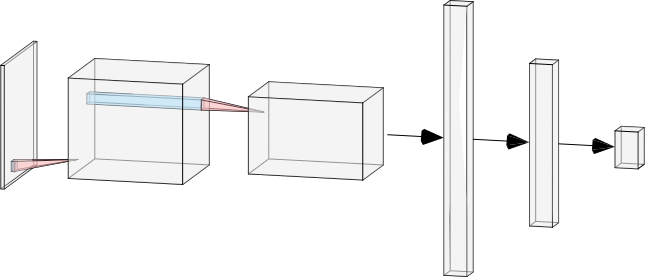
\includegraphics[width=.9\textwidth]{cnn.pdf}
        };

        \node at (1,-0.5) {Convolution};
        \node at (5,-0.5) {Convolution};
        \node at (9.5,-0.5) {Flatten};
        \node at (11.8,-0.5) {Dense};
        \node at (14,-0.5) {Dense};

        \node at (0.3,7) {$40\times40\times1$};
        \node at (3.3,6) {$20\times20\times32$};
        \node at (7.4,7) {$10\times10\times32$};
        \node at (10.8,7) {$3200$};
        \node at (12.8,7) {$128$};
        \node at (14.9,7) {$3$};
    \end{tikzpicture}
\end{frame}

\begin{frame}
    \frametitle{Segmentierung - Punktweise}
    \setlength{\tabcolsep}{1pt}
    \hspace*{-1.8cm}
    \begin{tabular}{c|rrrrrr}
        \toprule
        \diagbox{Predicted}{Actual} & \multicolumn{2}{c}{Ground} & \multicolumn{2}{c}{Foreground} & \multicolumn{2}{c}{Sparse} \\
        \midrule
        Ground & 958,704 & (92.1\%) & 3,436 & (2.0\%) & 12,224 & (53.3\%) \\ 
        Foreground & 70,293 & (6.8\%) & 164,209 & (97.9\%) & 10,416 & (45.4\%)  \\ 
        Sparse & 11,688 & (1.1\%) & 71 & (0.04\%) & 273 & (1.2\%) \\ 
        \midrule
        Gesamt & 1,040,685 && 167,716 && 22,913 \\
        \bottomrule
    \end{tabular}
\end{frame}

\begin{frame}
    \frametitle{Segmentierung - Zellenweise}
    \setlength{\tabcolsep}{3pt}
    \hspace*{-1.6cm}
    \begin{tabular}{c|rrrrrr}
        \toprule
        \diagbox{Predicted}{Actual} & \multicolumn{2}{c}{Ground} & \multicolumn{2}{c}{Foreground} & \multicolumn{2}{c}{Sparse} \\
        \midrule
        Ground & 8,302 & (96.9\%) & 45 & (14.8\%) & 227 & (0.45\%) \\
        Foreground & 184 & (2.1\%) & 248 & (81\%) & 45 & (0.1\%) \\
        Sparse & 79 & (0.92\%) & 12 & (4.0\%) & 49,943 & (99.5\%) \\
        \midrule
        Gesamt & 8,565 && 305 && 50,215 \\
        \bottomrule
    \end{tabular}
\end{frame}

\begin{frame}
    \frametitle{Clustering und Bounding-Box Schätzung}
    \begin{columns}
        \begin{column}{.5\textwidth}
            \begin{tabular}{cc}
                \toprule
                Durchschnitt 2D & 0.444 \\
                Durchschnitt 3D & 0.321 \\
                \bottomrule
            \end{tabular}
        \end{column}
        \begin{column}{.5\textwidth}
            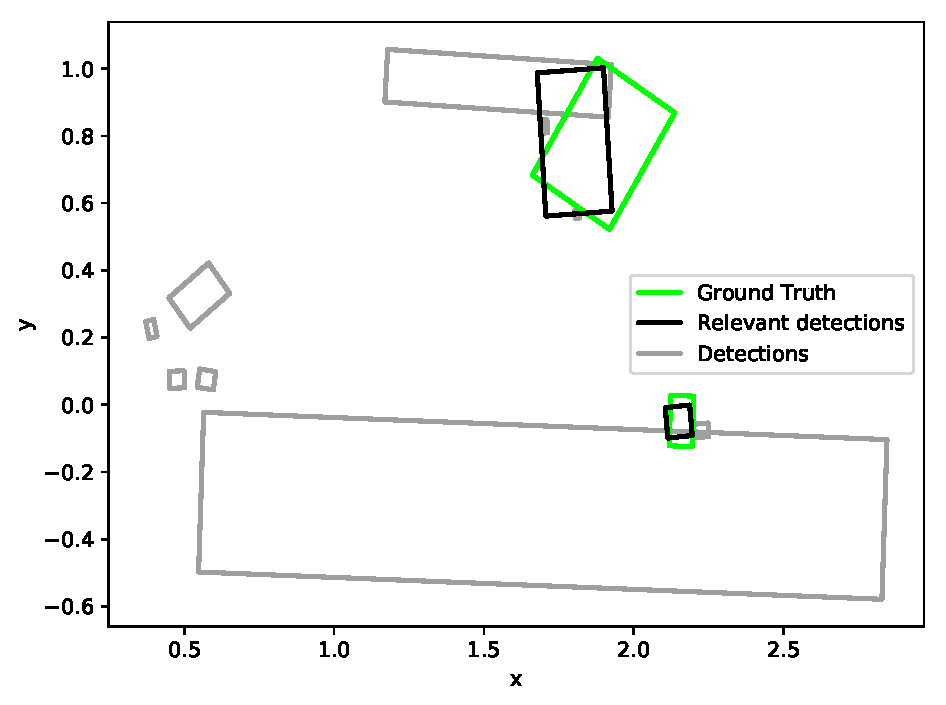
\includegraphics[width=\textwidth]{../Materalien/iou0.pdf}
            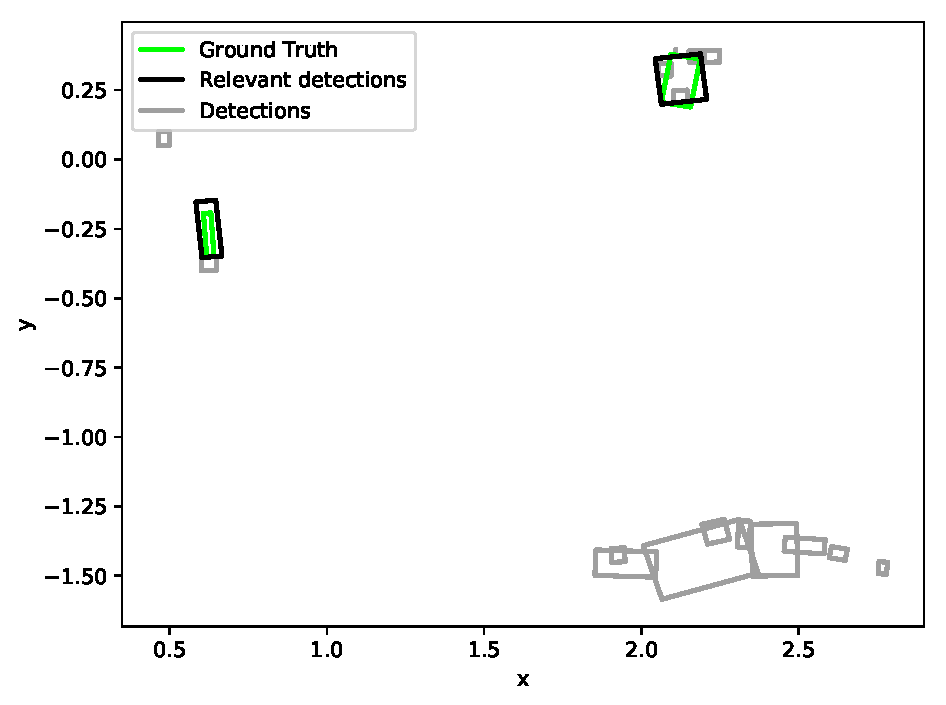
\includegraphics[width=\textwidth]{../Materalien/iou2.pdf}
        \end{column}
    \end{columns}
\end{frame}

\begin{frame}
    \frametitle{Klassifikation}
    \setlength{\tabcolsep}{3pt}
    \hspace*{-1.0cm}
    \begin{tabular}{c|rrrrrr}
        \toprule
        \diagbox{Predicted}{Actual} & \multicolumn{2}{c}{Clutter} & \multicolumn{2}{c}{Obstacle} & \multicolumn{2}{c}{Sign} \\
        \midrule
        Clutter & 555 & (89.5\%) & 3 & (15.8\%) & 3 & (16.7\%) \\
        Obstacle & 49 & (7.9\%) & 15 & (78.9\%) & 1 & (5.6\%) \\
        Sign & 16 & (2.5\%) & 1 & (5.2\%) & 14 & (77.8\%) \\
        \midrule
        Gesamt & 620 && 19 && 18 \\
        \bottomrule
    \end{tabular}
\end{frame}

\begin{frame}
    \frametitle{Evaluation - Verbesserungen}
    \hspace*{-0.5cm}
    Vorgeschlagen:

    \hspace*{-0.5cm}
    \begin{tabular}{c|c|rrr}
        \toprule
        Kategorie & Anzahl & Pr & Rc & $F_1$\\
        \midrule
        Obstacle/Pedestrian & 20 & 100\% & 84\% & 91\% \\
        Sign & 18 & 78\% & 100\% & 88\% \\
        \midrule
        Durchschnitt/Summe & 38 & 89\% & 92\% & 90\% \\
        \bottomrule
    \end{tabular}

    \vspace{0.5cm}
    \hspace*{-0.5cm}
    \cite{AttBen17}:

    \hspace*{-0.5cm}
    \begin{tabular}{c|c|rrr}
        \toprule
        Kategorie & Anzahl & Pr & Rc & $F_1$\\
        \midrule
        Obstacle/Pedestrian & 20 & 100\% & 80\% & 89\% \\
        Sign & 17 & 71\% & 100\% & 83\% \\
        \midrule
        Durchschnitt/Summe& 37 & 86\% & 90\% & 86\% \\
        \bottomrule
    \end{tabular}
\end{frame}

\begin{frame}
    \frametitle{Bodenschätzung}
    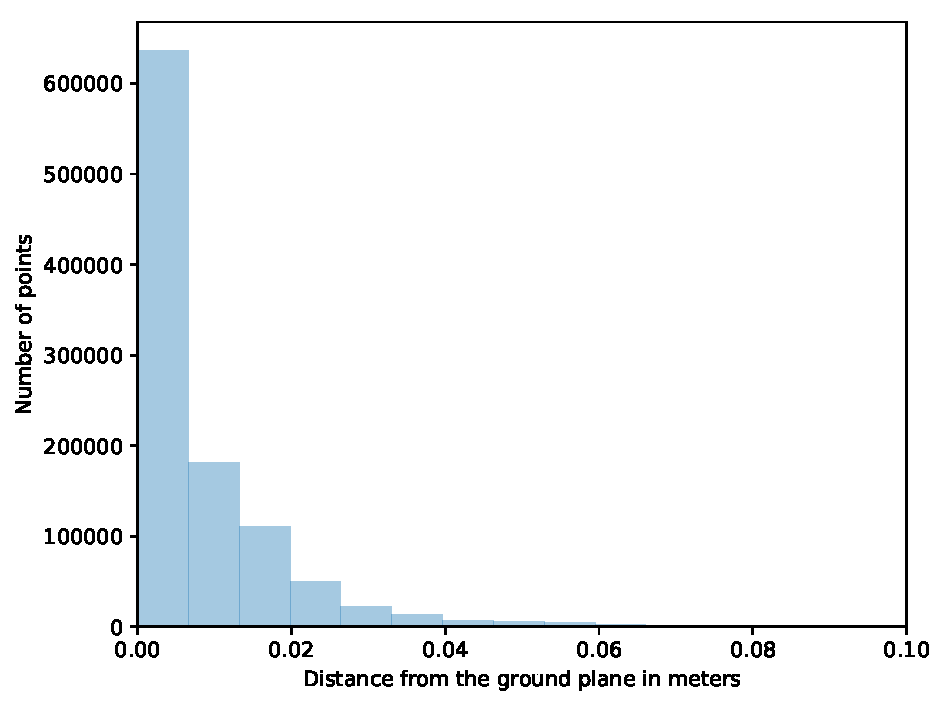
\includegraphics[width=\textwidth]{../Materalien/ground.pdf}
\end{frame}

\begin{frame}
    \frametitle{Evaluation Lehr}
    \begin{columns}
        \begin{column}{.5\textwidth}
            \begin{tabular}{cc}
                \toprule
                Durchschnitt 2D & 0.53\\
                Durchschnitt 3D & 0.43 \\
                \bottomrule
            \end{tabular}
        \end{column}
        \begin{column}{.5\textwidth}
            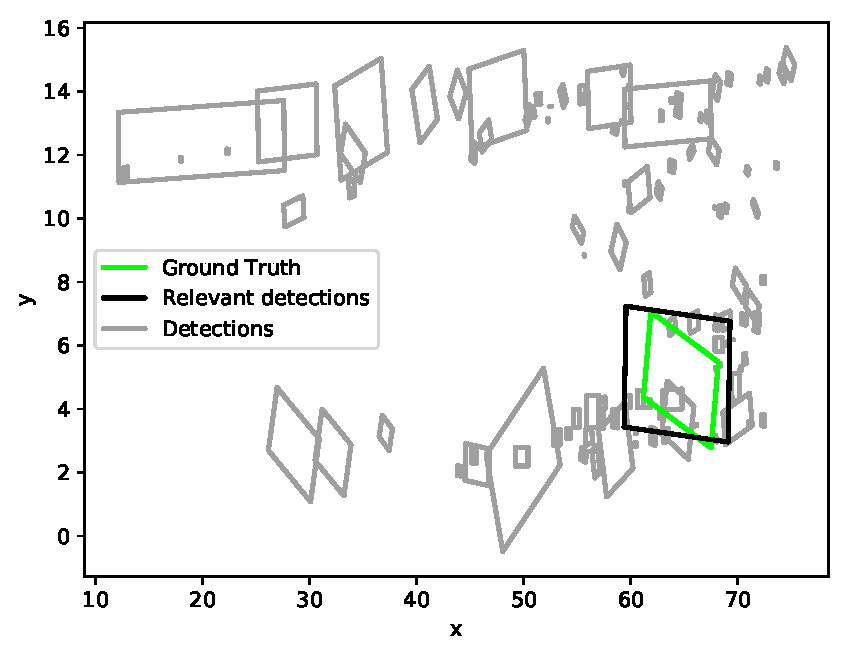
\includegraphics[width=\textwidth]{../Materalien/lehr1.pdf}
            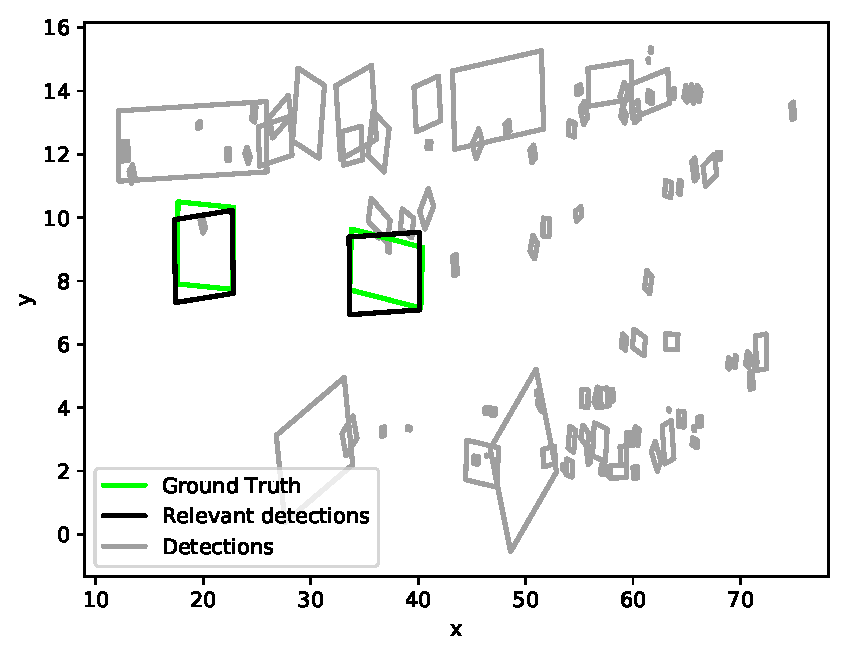
\includegraphics[width=\textwidth]{../Materalien/lehr2.pdf}
        \end{column}
    \end{columns}
\end{frame}
